\chapter{地面效应下的执行器控制效益离线辨识}
风扇在靠近地面飞行时的不稳定特性显著，可能导致稳定性问题。

\section{模型建立} % 3 Pages
\label{sec:model_identification}
精确的数学模型是进行控制器设计与系统分析的基础。本章针对涵道式无人机在近地面飞行时所受到的地面效应影响，建立推力和控制力矩的数学模型。鉴于地面效应的复杂流动机理，本章采用半经验模型与实验数据相结合的方法，分别构建适用于控制器设计的推力衰减模型与控制力矩插值模型。

\subsection{推力模型}

涵道风扇在靠近刚性平面工作时，其推力特性会因地面效应而发生显著变化。与孤立螺旋桨类似，地面的存在改变了涵道风扇的入流与尾流场分布，导致其气动特性与开放空间迥异\cite{matuz2021ground}。为量化这一影响并服务于无人机的高度控制，本节建立地面效应下的涵道风扇推力模型。

为描述无人机距离地面的相对高度，引入无量纲高度参数$h/R$，其中$h$为涵道出口平面距离地面的垂直距离，$R$为涵道风扇的半径。该参数是衡量地面效应强度的关键特征量。根据现有研究，对于涵道式风扇，由于其涵道壁对气流的约束作用，地面效应的影响范围可延伸至$h/R = 4.0$，当$h/R > 4.0$时可视为无地效区\cite{MI2020105821, matuz2021ground}。此外，当$h/R < 0.2$时，叶片尖端会发展出大量失速涡胞，导致气流泄漏显著增加，旋翼推力急剧下降，且流场呈现强烈的非定常特性，时间平均推力模型的预测精度难以保证\cite{luo2023numerical}。因此，本文所建立的推力模型适用范围为$0.2 \leq h/R \leq 4.0$，该区间涵盖了无人机起飞、降落及低空悬停的主要工况。

地面效应对涵道风扇推力的影响机理可归纳如下：高速旋转的桨叶将气流加速并经由涵道排出，形成向下的射流。当无人机接近地面时，该射流撞击地面后受阻并向四周径向扩散。这一过程在涵道出口与地面之间形成高压区，导致涵道出口背压升高\cite{luo2023numerical, MI2020105821}。高压区的存在对涵道风扇的各部分产生了不同的影响：一方面，地面阻塞效应使得涵道出口静压升高，增加了涵道壁产生的推力；另一方面，由于出口气流受阻，螺旋桨盘处的诱导速度发生变化，导致螺旋桨自身的拉力有所下降\cite{luo2023numerical, Bai2025}。两者的耦合作用决定了涵道风扇总推力的变化趋势。此外，撞击地面后反弹的气流会向上卷起，在涵道周围形成地面涡，部分涡流甚至会被重新吸入涵道，进一步影响涵道内部的流场结构\cite{luo2023numerical}。

上述复杂的流动机理使得纯粹基于物理的解析建模极为困难。因此，本文采用目前地面效应研究中广泛应用的半经验模型来描述推力的变化规律\cite{matuz2021ground}。该模型将地面效应下的推力$T_{\mathrm{GE}}$表示为无地效推力$T_{df}$与一个无量纲系数的乘积：
\begin{equation}
    T_{\mathrm{GE}} = C_{\mathrm{GE}} \cdot T_{df},
\label{eq:thrust_model}
\end{equation}
其中，$C_{\mathrm{GE}}$为地面效应推力系数，它仅是无量纲高度$h/R$的函数，反映了地面效应对推力的调制作用。将式\eqref{eq:thrust}代入式\eqref{eq:thrust_model}，可得：
\begin{equation}
    T_{\mathrm{GE}} = \frac{1}{2}T_{\mathrm{GE}} \rho \pi C_T R^4 \Omega^2
\end{equation}

推力系数$C_{\mathrm{GE}}$的数学表达应满足两个基本的物理约束：其一，当无人机远离地面时，地面效应应趋于消失，即满足$\lim_{h/R \to \infty} C_{\mathrm{GE}} = 1$；其二，在近地面区域，$C_{\mathrm{GE}}$应能准确反映推力的实际变化趋势。基于以上考虑，并参考现有文献中对涵道风扇及旋翼地面效应的研究成果\cite{luo2023numerical, MI2020105821, matuz2021ground}，本文采用指数衰减模型来描述$C_{\mathrm{GE}}$：
\begin{equation}
C_{\mathrm{GE}} = C_{\mathrm{amp}} \cdot e^{-C_{\mathrm{exp}} \cdot (h/R)} + 1.
\label{eq:ge_coefficient}
\end{equation}
式中，$C_{\mathrm{amp}}$为幅值系数，决定了地面效应的最大影响程度；$C_{\mathrm{exp}}$为指数衰减系数，控制着$C_{\mathrm{GE}}$随高度增加的衰减速率。式\eqref{eq:ge_coefficient}中的常数项$1$保证了当$h/R \to \infty$时，$C_{\mathrm{GE}}$收敛于1，使模型满足无地效极限。该模型结构简洁，参数具有明确的物理意义，已被研究证实能够有效拟合实验数据\cite{matuz2021ground}。例如，文献\cite{luo2023numerical}通过对涵道风扇地面效应的CFD仿真数据进行拟合，得到了形如式\eqref{eq:ge_coefficient}的指数模型，其拟合优度$R^2$达到0.9926，验证了该模型的有效性。

需要指出的是，本节所建立的推力模型侧重于描述推力的时间平均特性。尽管近地面流场存在固有的非定常波动，例如叶片通过频率引起的周期性推力脉动及失速涡胞的迁移等\cite{luo2023numerical}，但考虑到本文的研究重点在于高度控制器的设计，平均推力模型已能反映主导的静态增益变化，为控制器提供必要的模型补偿。具体的参数$C_{\mathrm{amp}}$与$C_{\mathrm{exp}}$将通过第\ref{sec:GE_exp}节的地面效应台架实验数据进行辨识确定。

\subsection{控制力矩模型}

由于无人机在近地面时，从涵道出口排出的高速气流撞击地面后，会向四周扩散并形成径向射流，靠近涵道出口中心的下洗气流因地面阻塞而形成流速极低的“死水区”。导致有效气流面积减小，气流紊乱，致使产生的升力下降。
尽管气流相对紊乱，但是可以确定的是，在相同气流环境下，舵面能够产生的升力是与舵面角度大致成线性关系的。
且考虑到远离地面过程中，地面效应带来的衰减将趋近于零，因此可以假设控制舵面满足如下关系
\begin{equation}
    F_{cvi} = C_{\mathrm{cvGE}} \cdot F_{cvi}
\end{equation}

\begin{figure}
    \centering
    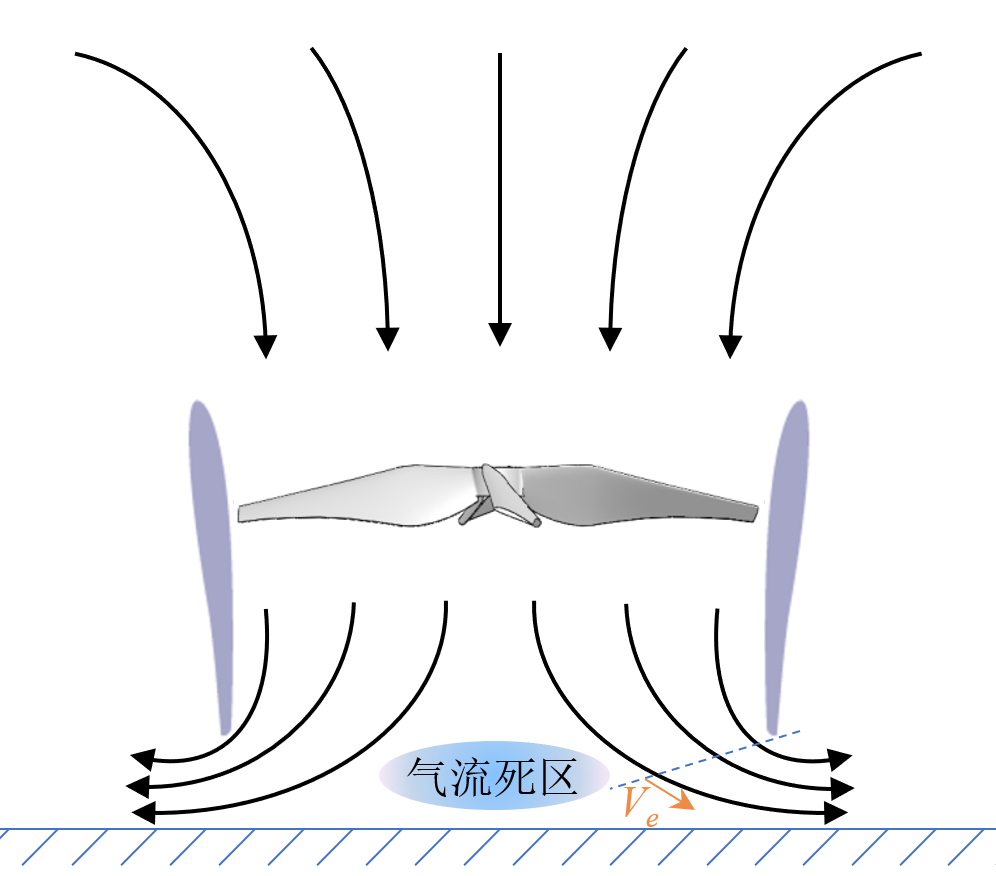
\includegraphics[scale=0.3]{figure/chapter4/ground_effect_flow.png}
    \caption{地面效应下气体流动示意图}
\end{figure}




\section{实验平台} % 1 Page
\label{sec:exp_platform}
为准确获取涵道式无人机在地面效应影响下的执行器效率与控制力矩特性，并为第\ref{sec:model_identification}节中的参数拟合提供可靠的实验数据，本文搭建了一套基于多轴力/力矩传感器的变高度静态测试台架。通过该平台开展的静态台架实验，旨在完成对涵道风扇推力效益及控制舵面力矩效益的地面标定，从而建立地面效应下执行器控制效益的数学模型。

实验平台的机械结构如图\ref{fig:experiment_platform}所示。台架主体采用铝合金型材搭建，具有足够的结构刚度以保证测试过程中的稳定性。上方采用龙门架结构固定一块面积远大于涵道风扇出口截面的刚性约束板，用于模拟真实的地面。该约束板可沿固定在龙门架两侧的精密竖直导轨平稳滑动，以精确调节其与涵道风扇之间的垂直距离。导轨上附有高精度直尺，用于记录每次数据采集时的约束板位置，从而确定离地高度。为保证实验数据的准确性与可重复性，实验中对离地高度$h$作如下定义：无人机底部支撑脚所在平面至约束板上表面的垂直距离。实验涵盖的无量纲高度范围为$0.2 \leq h/R \leq 5.0$，其中$R$为涵道风扇半径，该范围完整覆盖了从强地面效应区到无地效区的过渡。

实验样机以倒置姿态固定于测试台架上。具体而言，无人机机身通过专用夹具与下方的六维力/力矩传感器刚性连接，传感器则固定于底部基座上。采用倒置安装方式可使涵道风扇产生的推力垂直向上作用于传感器，便于直接测量。为准确获取螺旋桨的真实转速，排除了因供电电压波动或电机个体差异导致的转速不确定性，实验中使用高精度无刷电机转速传感器实时采集电机的电频率信号，并换算为螺旋桨的机械转速。整个实验系统由可编程数字直流电源供电，确保在长时间、多工况的测试过程中，供电电压保持稳定，从而保证电机工况的一致性和传感器数据的可靠性。

力/力矩传感器是本次实验的核心测量设备。根据实验样机在悬停及近地面工况下的预估最大推力与力矩，选用了量程合适、精度满足要求的传感器型号。传感器可同时测量三轴力与三轴力矩，其采样频率设置为$200\mathrm{Hz}$。这一采样频率，使得后期数据处理时可通过时域平均有效滤除高频噪声与气流脉动带来的随机误差，从而获得高精度的稳态气动力数据。

通过上述实验平台，可开展两类核心测试：一是地面效应下的涵道风扇推力效益测试，旨在获取不同离地高度下风扇推力相对于无地效状态的增益或损失；二是地面效应下的控制舵面力矩效益测试，旨在获取不同离地高度下各舵面单位偏角所产生的控制力矩。两类实验的具体步骤与数据处理方法将在后续章节详述。

\begin{figure}
    \centering
    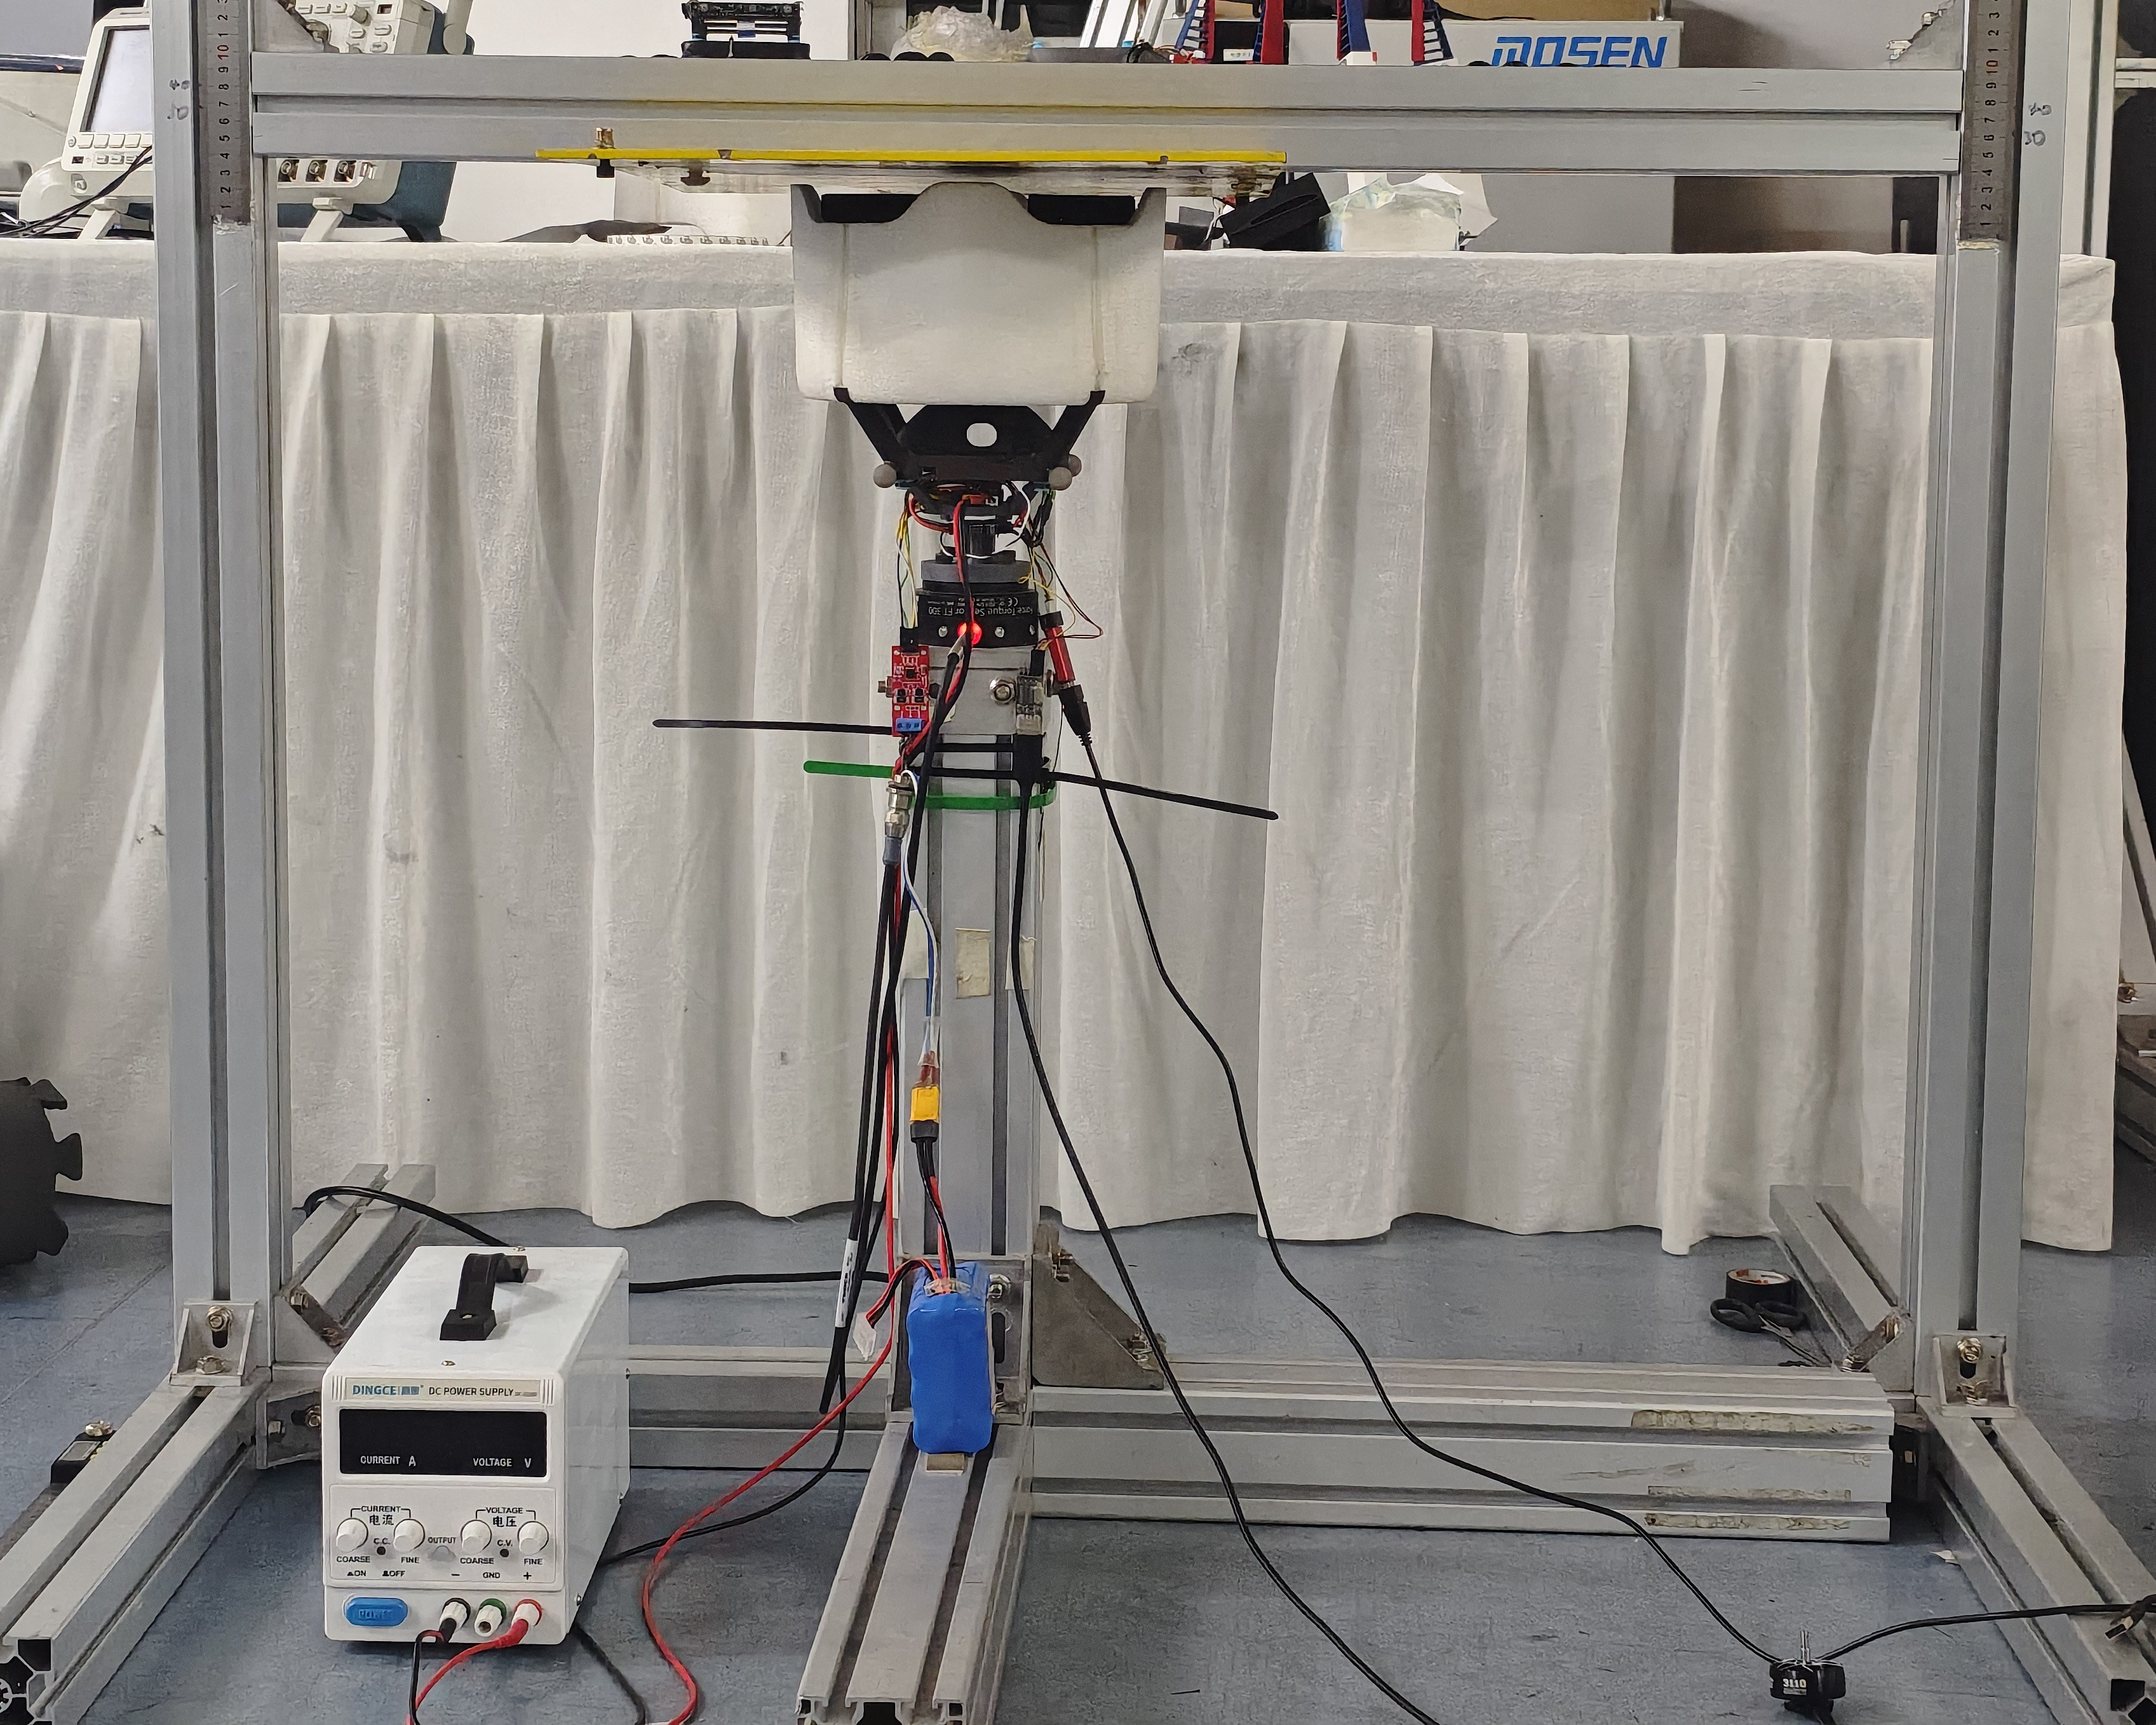
\includegraphics[width = 0.65\textwidth]{figure/chapter4/ground_effect_platform.jpg}
    \caption{\label{fig:experiment_platform}地面效应数据采集实验平台}
\end{figure}

\section{ 地面效应下涵道风扇推力效益测试}
\label{sec:GE_exp}
\subsection{实验步骤} % 2 Pages
由于力传感器存在较大的测量噪声，且无人机旋转过程中产生较大幅度的震动，因此需要对力传感器测量值进行均值处理。

力传感器存在静态误差，且需要排除无人机自身重量导致传感器无法测量出螺旋桨和控制舵面产生的推力和扭矩，因此，在实验开始之前，需要采集力传感器的静态输出力和力矩，并在结束时将该静态输出减去。

将无人机固连在力传感器上。使用数字电源供电
依次将挡板固定在不同高度上，并给电机由低到高发送油门指令，驱使螺旋桨达到不同转速。
在发出油门信号的2s后，认为电机旋转至平稳状态，记录力传感器数据。
将力传感器数据记录在飞控板的机载SD卡上。

\subsection{实验数据} % 2 Pages
按照上述实验步骤将数据采集之后，即可得到推力$T$和离地高度$h$以及涵道风扇转速$\Omega$之间的关系。

\begin{figure}
    \centering
    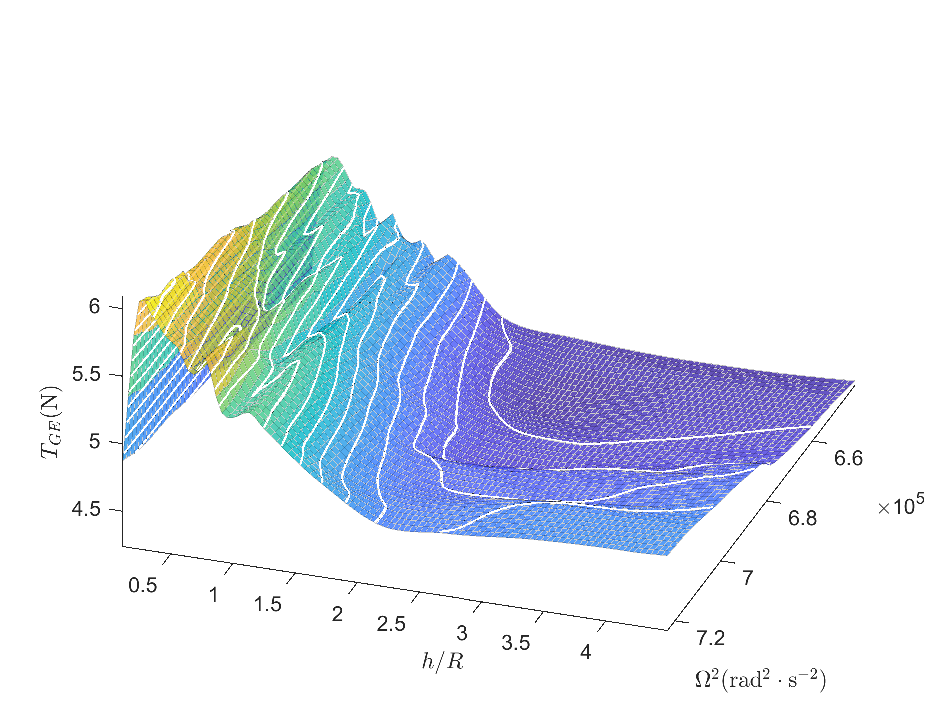
\includegraphics{figure/chapter4/surf_T-omega-h.pdf}
    \caption{\label{fig:T-omega-h}涵道风扇推力和风扇转速、离地高度之间的关系}
\end{figure}

本文从两个维度来观察该实验结果，分别是在指定高度下，推力随涵道风扇转速变化的曲线；以及在指定涵道风扇转速下，推力随高度变化的曲线。

\begin{figure}[htbp]
    \centering
    \begin{minipage}[b]{0.45\textwidth}
        \centering
        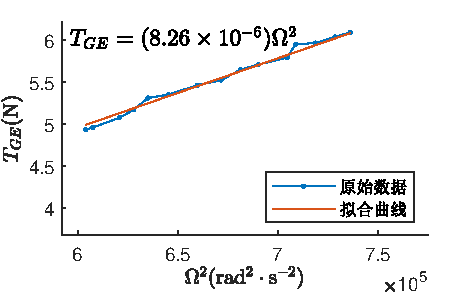
\includegraphics{figure/chapter4/rotor_thrust_30mm.pdf}
        \caption*{$h = 30 \mathrm{mm}$}
    \end{minipage}
    \hfill  % 产生弹性水平间距
    \begin{minipage}[b]{0.45\textwidth}
        \centering
        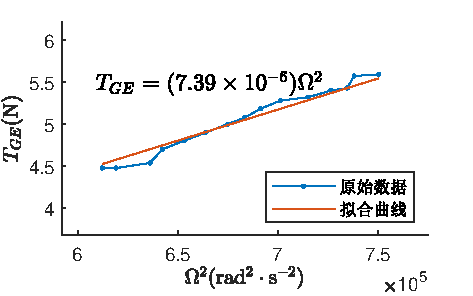
\includegraphics{figure/chapter4/rotor_thrust_100mm.pdf}
        \caption*{$h = 100 \mathrm{mm}$}
    \end{minipage}

    \vspace{0.5cm}

    \centering
    \begin{minipage}[b]{0.45\textwidth}
        \centering
        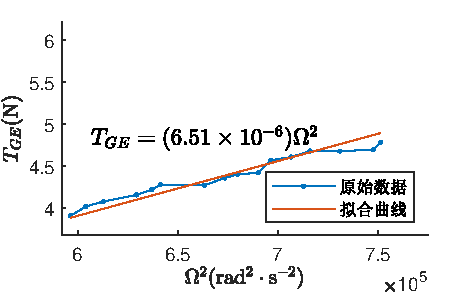
\includegraphics{figure/chapter4/rotor_thrust_200mm.pdf}
        \caption*{$h = 200 \mathrm{mm}$}
    \end{minipage}
    \hfill  % 产生弹性水平间距
    \begin{minipage}[b]{0.45\textwidth}
        \centering
        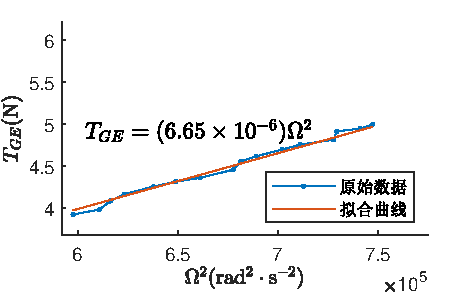
\includegraphics{figure/chapter4/rotor_thrust_400mm.pdf}
        \caption*{$h = 400 \mathrm{mm}$}
    \end{minipage}
    \caption{不同高度$h$下推力$T$与风扇转速$\Omega$的关系}
\end{figure}

可见在不同高度下，即使推力受到较大影响，推力和螺旋桨转速的平方仍然呈现出正比例关系，这也从侧面印证了模型\eqref{eq:thrust_model}建立的合理性。
此外，不难看出，离地面越近时，无人机受到的推力越大，其推力提高随油门上升的程度也越大（此处需要引用参考文献的说法描述其机理）。

在典型悬停转速下，分析风扇推力和离地高度的关系：

\begin{figure}[htbp]
    \centering
    \begin{minipage}[b]{0.45\textwidth}
        \centering
        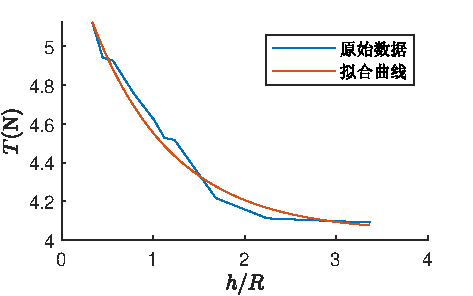
\includegraphics{figure/chapter4/line_T-h.pdf}
    \end{minipage}
    \hfill  % 产生弹性水平间距
    \begin{minipage}[b]{0.45\textwidth}
        \centering
        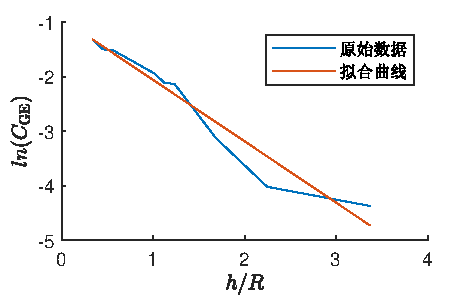
\includegraphics{figure/chapter4/line_ln_GE-h.pdf}
    \end{minipage}
    \caption{\label{fig:T-h}涵道风扇推力和离地高度的关系}
\end{figure}

\section{ 地面效应下控制舵面控制力矩效益测试}
\subsection{实验步骤} % 2 Pages
\subsection{实验数据} % 2 Pages

\section{控制效应参数拟合} % 3 Pages
\label{sec:exp_identification}
\subsection{数据预处理}
\subsection{参数拟合}


\section{本章小结} % 1 Pages